
\documentclass[12pt]{article}
%	options include 12pt or 11pt or 10pt
%	classes include article, report, book, letter, thesis

\usepackage[margin=0.5in]{geometry}
\setlength{\parindent}{0pt}

\usepackage{hyperref}
\usepackage{enumerate}
\usepackage{graphicx}

%for writing of code in blocks like
%\begin{lstlisting}
%   .......
%\end{lstlisting}
\usepackage{listings}
\usepackage{color}

\definecolor{dkgreen}{rgb}{0,0.6,0}
\definecolor{gray}{rgb}{0.5,0.5,0.5}
\definecolor{mauve}{rgb}{0.58,0,0.82}

\lstset{frame=tb,
  language=C++,
  aboveskip=3mm,
  belowskip=3mm,
  showstringspaces=false,
  columns=flexible,
  basicstyle={\small\ttfamily},
  numbers=none,
  numberstyle=\tiny\color{gray},
  keywordstyle=\color{blue},
  commentstyle=\color{dkgreen},
  stringstyle=\color{mauve},
  breaklines=true,
  breakatwhitespace=true,
  tabsize=3
}
%%%%%%%%%%%%%%%%%%%%%%

\title{Particle Physics : Throwing Dice and Skwigly Lines}
\author{Sam Meehan and Eric Rasco}
\date{21 December 2017}

\begin{document}
\maketitle

\textbf{Notes}
\begin{itemize}
\item You should submit your work for both activities in the format of short report (for each) that includes four sections : \textit{(i)} a description of the activity and why you are doing it \textit{(ii)} a description of the procedure you followed in the activitiy \textit{(iii)} the data you took, in the form of a table of measurements, a graph, a histogram, a visual drawing etc. \textit{(iv)} a conclusion describing what you learned from the activity.
\item At the top of the paper you should write your name, the date, and whether you prefer milk or dark chocolate. 
\end{itemize}


\textbf{Activity 1 - Who ordered that?!? - Probability and Quantum Stuff}
\newline
In this activity, we will investigate the idea of probability in the context of flipping coins, throwing dice, and then something a bit funkier; measuring the position of a particle in a box (maybe not so funky)!  The mathematical concept of probability and statistics is central to particle physics and is what allows scientists working at CERN to summarize tons of data coming from their experiments into meaningful statements about the fundamentals of nature. Try to figure out how much data comes from these experiments based on this description.  Collisions at the Large Hadron Collider machine, happen once every 25 ns during 8 months out of the year.  During these 8 months, the machine operates in periods of 8 hours on and 2 hours off.  The ATLAS experiment produces measurements from $\sim$100 million individual detectors during each collision.  Each of these individual detectors represents one decimal point number which is equivalent to 32 \textit{bytes}\footnote{This is like the \textit{byte} in Giga-\textit{byte} on your computer, but only 32 of them, not one million of them!}.  So how much data is produced by this experimente each year?
\newline
\newline
In this activity, you will study the statistical behavior of three different systems and summarize their behavior using a histogram.  Most importantly, you will attempt to quantify the \textit{uncertainty} on your measurements - without uncertainty, a measurement to a particle physicist is typically not terribly meaningful.  
\newline
\newline
\textbf{Coin Flipping}
\newline
Get a coin from the teacher.  Don't flip it yet but describe it.  If you were to flip it and let it land without touching it, what would be the possible outcomes?  Do you think that one of these outcomes is more likely to happen than another?  What are the features of the coin that lead you to your conclusion? (This is called a \textit{Gedankenexperiment}, which is German for “thought experiment” and is what we use to build our intuition and expectation for what should happen in a physical experiment - the most important thing is to then test this expectation with a real experiment.)
\newline
\newline
Now flip the coin once and record in a table whether it is heads or tails.  Based on this single flip, are you able to say if it is more likely to have appeared as heads or tails? Make a histogram of this single experiment of one flip.  It should have two columns (one heads, one tails). 
\newline
\newline
Now flip the coin 5 times and again make a histogram of the outcomes.  Are you able yet to tell if the coin is a \textit{fair} coin?  What would you need to observe for it to be a fair coin?  Can this happen when flipping the coin 5 times?
\newline
\newline
Now flip the coin 10 times and make a histogram of the outcomes.  If the number of heads and tails is not the same, can you conclude that the coin is not a \textit{fair} coin?  To help us do this, let's quantify the uncertainty on your measurements.  Now, there is a bit of mathematics involved here, but what we are doing is a \textit{counting experiment} and in general for experiments like this, the probability to get a certain outcome is described by a ``Poisson'' (not fish) distribution and the uncertainty on either one of your measurements is equal to the square root of the number of counts of that type.  So, if you got 4 heads, then the uncertainty on that is 2.  Knowing this, improve your histogram representation of the data by adding uncertainties to each of the columns.  Now ask yourself the same question, ``Is this coin a fair coin?'' this time being wary of the fact that fair does not mean if the number of heads is the same as the number of tails but whether the two error bars overlap.
\newline
\newline
Finally as yourself, what would happen to the size of the error bars (\textit{absolute error}) if you were to increase the number of times you flipped the coin?  Would they increase or decrease?  What would happen to the ratio of the size of the error bars to the total counts (\textit{relative error}) if you were to increase the number of times you flipped the coin?
\newline
\newline
\textbf{Dice Rolling}
\newline
We will now perform a similar, but slightly more complicated experiment using a dice.  Get a dice from the teacher.  Again, don't roll the dice but take it and describe the possible outcomes \textit{if you were to roll it}.  Like the dice, should any of the 6 sides be preferred over the others?  If the dice is a fair dice, what would you expect when you roll it?
\newline
\newline
Now start rolling the dice.  Roll the dice 6 times and make a histogram of the outcomes (include your error bars!).  Can you say if the dice is fair or not?  Repeat this experiment but with more data.  Roll the dice 10 times, then 60, and finally  120 times.  Based on your data, can you conclude that your dice is a fair dice?
\newline
\newline
\textbf{Particle in a Box}
\newline
Finally, we will perform a quantum experiment on the computer.  The setup of the experiment is that we have a particle in a box, like in Fiure~\ref{fig:box}.  This is one of the simplest experiments that exists in quantum physics.  
\begin{figure}[!ht]
\centering
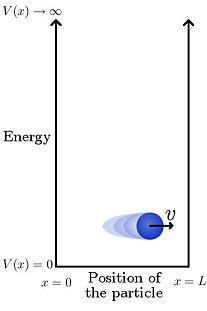
\includegraphics[width=0.2\textwidth]{pib.jpg}
\caption{A classical example of a particle (the blue ball) in a ``box'' which is formed by a potential energy barrier of infinite strength.}
\label{fig:box}
\end{figure}
\newpage
Hopefully you have gotten good as thinking about Gedankenexperiments because we now must ask ourselves what we expect to see here.  Let's pretend that we close our eyes and let the particle move back and forth in the box and then at some random time, whenever you feel like it or when a friend tells you to do so, you open your eyes and observe and record the position \textit{x} of the ball.  You then close your eyes and do it again ... and again, and again ... If you were to make a histogram of the position of the ball, what would you expect to see?  Sketch your expectation.
\newline
\newline
Do you think this same intuition/expectation holds if the particle in question is now not a blue ball, but a single electron particle?  That is what we will test - but to run this experiment, we need to use a computer.
\newline
\newline
Open your computer terminal (ask the teacher if you don't know what this means) and type the following command :
\newline
\begin{lstlisting}
python ParticleInBox.py
\end{lstlisting}

What is printed out on the screen is a measurement of the position \textit{x} of the electron in a box that is much much smaller than the one drawn above and runs from $x=$0$nm$ to $x=$10$nm$.  This time, since we are actually doing the experiment, record this measurement and repeat the experiment.  You will again want to create a histogram to represent your data but this time, the measurement is not divided up so nicely into two or six regions, so you will have to make \textit{bins} to categorize your measurements.  If a single measurement falls within the bounds of one of the bins, then add a count to that bin.  Divide the region into 10 bins and start building your histogram.  You will need to perform this experiment at least one hundred times to start to come to a conclusion about whether your expectation is correct.  Be sure to put error bars on your histogram after you are finished making your measurements!

Is this system of an electron in a very tiny box behaving as you expect?  If not, describe an interesting feature that you observe.  

\newpage
\textbf{Activity 2 - Surely you are joking Mr. Feynman! Particle Physics with Pictures}
In this activity, you will work to understand how to model particle physics using what are called ``\textit{Feynman diagrams}''.  Particle physics is the study the interactions of what we believe to be the smallest particles that exist (like the electrons you dealt with in Activity 1) and due to this fact, they obey the laws of quantum physics.  This fundamentally means that what happens \textit{cannot} be predicted on a case-by-case basis, just like flipping a coin or rolling a dice.  Now, to study these interactions, what phsicists do is ``collide'' (smash together) two well-understood particles (like an electron $e^{-}$ and a positron $e^{+}$) and examine what comes out.  One way to think of this is as in Figure~\ref{fig:fd1} where we see the to input particles that will interact coming from the left and the resulting decay products coming out on the right.
\begin{figure}[!ht]
\centering
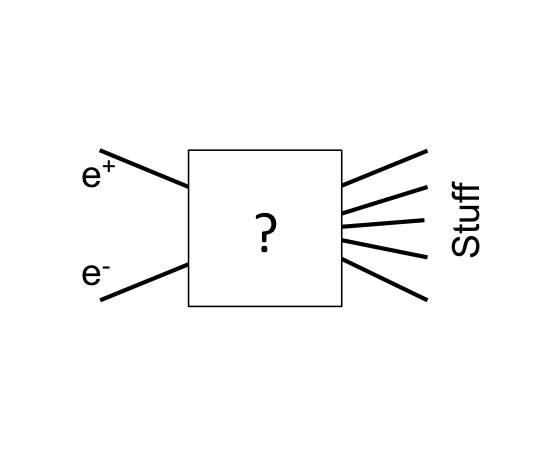
\includegraphics[width=0.4\textwidth]{fd1.png}
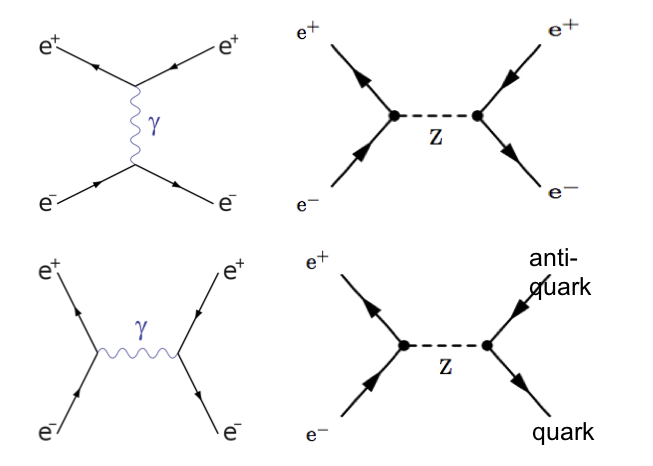
\includegraphics[width=0.4\textwidth]{fd2.png}
\caption{A schematic example of a collision of $e^{-}e^{+}$ to produce stuff (left) and a few examples of the type of things that may happen (right) such as the annihilation to a photon or the exchange of a photon ($\gamma$) or the creation of a $Z$ boson which can itself decay to $e^{-}e^{+}$ pair but also a quark/anti-quark pair ($q\bar{q}$).}
\label{fig:fd1}
\end{figure}
In the right of Figure~\ref{fig:fd1}, we can see a few examples of types of interactions.  Some of these can be written just like a chemical reaction.  For example, the annihilation of the $e^{-}e^{+}$ to a photon and its decay back to an $e^{-}e^{+}$ pair can be written like $e^{-}e^{+} \rightarrow \gamma \rightarrow e^{-}e^{+}$.  However, some of them, like the ``exchange'' of a photon is more challenging to write in such a straightforward manner.  However, we know from experiment that both of these processes \textbf{do} happen in real life - by which we mean collisions.  So, instead of using chemical equations, we use diagrams like this to represent the types of interactions.  

And the crazy thing about quantum physics is that anything can happen ... as long as you follow a few simple guidelines outlined below.
\begin{itemize}
\item The Ingredients
\begin{itemize}
\item \textbf{Propagators} : These are the lines (they may be straight or squigly) represent particles that come into existence or vanish when combined with another particle
\item \textbf{Vertices} : These are the dots where three lines come together into a single point and they represent interactions 
\end{itemize}
\item The Rules
\begin{itemize}
\item The propagators coming in from the left side of the page represent the input particles to the interaction.  These are the ones you control and choose when you design an experiment.
\item The propagators going out to the left that do not enter into any vertices represent the particles that will emerge from an interaction.  There is no need for these to be the same as the input particles!
\item Propogators cannot magically transform into a different propogator without going through an interaction with another propagator at a vertex.  This is the quantum version of Newton's first law (What was Newton's first law again?)\footnote{But like any set of rules there are always exceptions to the rule.  Study physics in college to learn these very very strange exceptions!}.
\item There are a fixed number of interaction vertices and strength of that type of vertex interaction is governed by something called the ``\textit{coupling}''.  This is analagous to the ``weighting'' of the quantum dice, so a vertex that has a high coupling is more likely to occur.
\item You can string together sets of vertices in any manor which obeys the fact that propagators do not change their identity magically.  And in fact in nature, every single possible diagram (of which there are a very large number; think infinity) occur at once.
\end{itemize}
\end{itemize}

So now, collect a bunch of vertices from your teacher and start to construct diagrams.  Can you construct two diagrams which are different but have the same input and output particles?  Which is more likely to occur?  Can you now construct a diagram that will transform two particles of some type into two particles of a different type - chemically speaking, can you create the reaction $e^{+}e^{-} \rightarrow XXX \rightarrow q\bar{q}$ ($XXX$ is what you will create)?  

\end{document}





















